% ============================================================
%  hw3_sol.tex   --  MATH 6660, Homework 3  (Problems 1-5).
%
%  RULE: nothing in this document goes beyond the class lectures.
%  Every step is tagged with the lecture it comes from.  Anything that
%  would go outside them is wrapped in \outside{}{} and prints as a red
%  labelled box, so it is visible in the PDF.
%
%  Build: pdflatex hw3_sol.tex   (twice, for cross-references)
% ============================================================
\documentclass[11pt]{article}
\usepackage[letterpaper,margin=1in]{geometry}
\usepackage[T1]{fontenc}
\usepackage{amsmath,amssymb,amsthm}
\usepackage{booktabs}
\usepackage{graphicx}
\usepackage{caption}
\usepackage{enumitem}
\usepackage{bm}
\usepackage{tikz}
\usetikzlibrary{arrows.meta}
\usepackage{xcolor}
\usepackage[colorlinks=true,linkcolor={blue!45!black},pdfborder={0 0 0}]{hyperref}
\usepackage{pdfcomment}
\usepackage{xspace}

\newcommand{\dx}{\,\mathrm{d}x}
\newcommand{\norm}[1]{\lVert #1\rVert}
\newcommand{\abs}[1]{\lvert #1\rvert}
\newcommand{\eps}{\varepsilon}
\newcommand{\ie}{i.e.\@\xspace}
\newcommand{\eg}{e.g.\@\xspace}
\setlength{\parindent}{0pt}

% ---- provenance tag: which lecture a step comes from ------------------
\newcommand{\src}[1]{{\small\color{black!55}\textsf{[#1]}}}

% ---- anything outside the lectures is boxed and labelled -------------
\newcommand{\outside}[2]{%
  \par\smallskip\noindent
  \fcolorbox{red!65!black}{red!4}{%
    \parbox{0.955\linewidth}{\small
      \textbf{\color{red!65!black}NOT FROM LECTURE --- #1}\par\smallskip #2}}%
  \par\smallskip}

% ---- bullets ---------------------------------------------------------
\newlist{steps}{itemize}{1}
\setlist[steps]{label=\textbullet, leftmargin=1.25em, topsep=3pt,
                itemsep=4pt, parsep=0pt}

% ---- hover tooltips on cross-references ------------------------------
\makeatletter
\newcommand{\settip}[2]{\expandafter\gdef\csname femtip@#1\endcsname{#2}}
\newcommand{\gettip}[1]{%
  \ifcsname femtip@#1\endcsname\csname femtip@#1\endcsname\else equation \ref{#1}\fi}
\newcommand{\eqr}[1]{\pdftooltip{\eqref{#1}}{\gettip{#1}}}
\makeatother

\settip{eq:bvp}{Cantilever beam: fourth derivative of u equals f, clamped at the left end, free at the right end}
\settip{eq:mult}{Multiply the beam equation by a test function v and integrate over the unit interval}
\settip{eq:ibp1}{After one integration by parts: boundary bracket of v times u triple prime, minus the integral of v prime u triple prime}
\settip{eq:ibp2}{After the second integration by parts: boundary bracket of v prime times u double prime, plus the integral of v double prime u double prime}
\settip{eq:weak}{Weak form: the integral of u double prime v double prime equals the integral of f v}
\settip{eq:V}{V is the set of v with v, v prime and v double prime square integrable, and v and v prime vanishing at the clamped end}

\begin{document}

\begin{center}
  {\large\bfseries MATH 6660 --- Homework 3}\\[2pt]
  {\normalsize Beam equation (cantilever)}\\[2pt]
  {\small Fall 2026}
\end{center}

\vspace{4pt}

{\small\color{black!60}
\textbf{Relation to the lectures.}  Lectures 10--11 derive the weak form of the
beam equation $u^{(iv)}=f$ and Lecture 12 carries CG(3) through to the assembled
system --- but for a beam \emph{clamped at both ends},
$u(0)=u(1)=u'(0)=u'(1)=0$.  This homework is the same beam with the right end
\emph{free}.  Only one thing changes: which of the four boundary terms are
killed by a condition on $v$ and which are killed by a condition on $u$.  The
machinery --- two integrations by parts, the space built from
$\int[v^{2}+(v')^{2}+(v'')^{2}]<\infty$, Hermite cubics, Galerkin orthogonality,
the duality argument --- is used exactly as the lectures state it.}

\vspace{4pt}

% ==================================================================
\section*{Problem 1}

\textbf{Problem.} Recast the cantilever beam problem as a variational problem.
Clearly state the test and trial function spaces.

\medskip
The strong problem is
\begin{equation}\label{eq:bvp}
  \left\{
  \begin{aligned}
    u^{(iv)}&=f(x), && x\in(0,1),\\
    u(0)=0,\quad u'(0)&=0, &&\text{(clamped end)}\\
    u''(1)=0,\quad u'''(1)&=0. &&\text{(free end)}
  \end{aligned}\right.
\end{equation}

% ------------------------------------------------------------------
\subsection*{Step 1 --- multiply by $v$ and integrate by parts twice
  \ \src{Lecture 11: same two steps, \ \ $\int v\,u^{(iv)}\to-\int v'u'''\to\int v''u''$}}

\begin{steps}
\item Multiply \eqr{eq:bvp} by a test function $v$ and integrate over $(0,1)$:
\begin{equation}\label{eq:mult}
  \int_{0}^{1} v\,u^{(iv)}\dx=\int_{0}^{1} f v\dx .
\end{equation}

\item First integration by parts:
\begin{equation}\label{eq:ibp1}
  \underbrace{\Bigl[v\,u'''\Bigr]_{0}^{1}}_{\text{bracket A}}
  \;-\;\int_{0}^{1} v'\,u'''\dx \;=\;\int_{0}^{1} f v\dx .
\end{equation}

\item Second integration by parts, applied to $-\int v'u'''$:
\begin{equation}\label{eq:ibp2}
  \text{bracket A}\;
  \underbrace{-\Bigl[v'\,u''\Bigr]_{0}^{1}}_{\text{bracket B}}
  \;+\;\int_{0}^{1} v''\,u''\dx\;=\;\int_{0}^{1} f v\dx .
\end{equation}
\end{steps}

% ------------------------------------------------------------------
\subsection*{Step 2 --- kill the two brackets
  \ \src{Lecture 6: Dirichlet $=$ essential, built into $V$; Neumann $=$ natural,
         no constraint on the space}}

Write the brackets out. Each has an $x=1$ half and an $x=0$ half, and the two
halves die for \emph{different reasons}:
\[
  \text{A}=\underbrace{v(1)\,u'''(1)}_{\text{$x=1$}}-\underbrace{v(0)\,u'''(0)}_{\text{$x=0$}},
  \qquad
  \text{B}=-\underbrace{v'(1)\,u''(1)}_{\text{$x=1$}}+\underbrace{v'(0)\,u''(0)}_{\text{$x=0$}} .
\]

\begin{center}\small
\renewcommand{\arraystretch}{1.3}
\begin{tabular}{@{}llll@{}}
\toprule
term & dies because & type & costs a condition on\\
\midrule
$v(1)\,u'''(1)$  & $u'''(1)=0$ is \emph{given} in \eqr{eq:bvp} & natural   & nothing\\
$v'(1)\,u''(1)$  & $u''(1)=0$ is \emph{given} in \eqr{eq:bvp}  & natural   & nothing\\
$v(0)\,u'''(0)$  & we \emph{impose} $v(0)=0$                   & essential & $v$\\
$v'(0)\,u''(0)$  & we \emph{impose} $v'(0)=0$                  & essential & $v$\\
\bottomrule
\end{tabular}
\end{center}

\begin{steps}
\item At the \textbf{free end} $x=1$ nothing is asked of $v$: the two boundary
      data $u''(1)=u'''(1)=0$ are already zero, so both $x=1$ halves vanish on
      their own.  This is Lecture 6's ``natural, weakly enforced, adds no
      constraint''.
\item At the \textbf{clamped end} $x=0$ the data $u'''(0)$ and $u''(0)$ are
      \emph{not} known --- they are the unknown reaction shear and reaction
      moment.  The only way to remove them is to demand $v(0)=v'(0)=0$.  This is
      Lecture 6's ``essential, strongly enforced, built into $V$''.
\item Both brackets are now zero, and \eqr{eq:ibp2} collapses to
\begin{equation}\label{eq:weak}
  \boxed{\;\int_{0}^{1} u''\,v''\dx=\int_{0}^{1} f\,v\dx\;}
\end{equation}
\end{steps}

% ------------------------------------------------------------------
\subsection*{Step 3 --- the space
  \ \src{Lecture 11, eq.~(1.170): same recipe, only the BC list is shorter}}

\begin{steps}
\item \eqr{eq:weak} asks for $\int (u'')^{2}$ and $\int (v'')^{2}$ to be finite,
      so the space is built on two derivatives --- exactly as in Lecture 11:
\begin{equation}\label{eq:V}
  \boxed{\;V=\Bigl\{v:\ \int_{0}^{1}\bigl[v^{2}+(v')^{2}+(v'')^{2}\bigr]\dx<\infty,
         \ \ v(0)=0,\ v'(0)=0\Bigr\}\;}
\end{equation}
\item Only the \emph{two} essential conditions appear in \eqref{eq:V}.  The
      lecture's clamped--clamped version lists four because that beam has two
      clamped ends; the cantilever has one.  The free-end conditions
      $u''(1)=u'''(1)=0$ are \textbf{not} written into $V$ --- they are already
      built into \eqr{eq:weak}, and a solution of \eqref{eq:weak} satisfies them
      whether or not anybody asks.
\item As in Lecture 11, functions in $V$ are $C^{1}[0,1]$: a corner in $v$ puts a
      jump in $v'$, hence a delta in $v''$, hence $\int (v'')^{2}=\infty$.
\end{steps}

% ------------------------------------------------------------------
\subsection*{Step 4 --- trial and test spaces
  \ \src{Lecture 5: trial $=$ test exactly when the essential BCs are homogeneous}}

\begin{steps}
\item \textbf{Trial space} $=V$.  The trial function is the unknown $u$; it must
      satisfy the essential conditions $u(0)=u'(0)=0$, and it must have finite
      bending energy $\int (u'')^{2}<\infty$.  That is \eqref{eq:V}.
\item \textbf{Test space} $=V$.  Step 2 forced $v(0)=v'(0)=0$ and \eqref{eq:weak}
      forced $\int (v'')^{2}<\infty$.  Same two requirements, same set.
\item They coincide because the essential BCs here are \emph{homogeneous}
      ($0$, not a prescribed settlement).  Lecture 5 is the case where they part:
      with $u(0)=\alpha\neq0$ the trial set is not even a vector space, and one
      uses $V$ for $u$ and $V_{0}$ for $v$.  That does not arise here.
\end{steps}

\medskip
\noindent\fbox{\parbox{0.955\linewidth}{%
\textbf{(Variational problem)}\ \ Find $u\in V$ such that
\[
  \int_{0}^{1}u''v''\dx=\int_{0}^{1}f v\dx
  \qquad\text{for all } v\in V,
\]
with $V$ given by \eqref{eq:V}, and trial space $=$ test space $=V$.}}

\medskip
{\small\color{black!60}\textbf{Mechanics reading.}  $\int u''v''$ is internal
virtual work (curvature $\times$ moment, with $EI\equiv1$); $\int fv$ is external
virtual work.  The statement is virtual work.  $v(0)=v'(0)=0$ says a virtual
displacement may not move or rotate the built-in end --- you cannot do virtual
work on a support.  Nothing is asked at the free tip because a free tip carries
no reaction.}

% ==================================================================
\newpage
\section*{Problem 2}

\textbf{Problem.} Interpret the variational problem as an energy minimization
problem, clearly stating the energy functional.  Prove that the variational
problem and the energy minimization problem are equivalent.

% ------------------------------------------------------------------
\subsection*{Step 1 --- the energy functional
  \ \src{Lecture 11, eq.~(1.171): $F(w)=\tfrac12\int(w'')^{2}-\int fw$ for this
         very beam}}

\begin{steps}
\item Lecture 3 built $F$ for the bar as \emph{internal energy} $-$ \emph{load
      potential}, $F(w)=\tfrac12\int a(w')^{2}-\int fw$ (eq.~1.29).  Lecture 11
      writes the beam version, one derivative higher:
\begin{equation}\label{eq:F}
  \boxed{\;F(w)=\underbrace{\frac12\int_{0}^{1}(w'')^{2}\dx}_{\text{bending strain energy}}
         \;-\;\underbrace{\int_{0}^{1}f\,w\dx}_{\text{load potential}}\;}
\end{equation}
\item $w''$ is the curvature, so with $EI\equiv1$ the first term is
      $\tfrac12\int EI\,\kappa^{2}$ --- the bending strain energy, as Lecture 11
      states.  $F$ is the total \emph{potential} energy $\Pi=U-W$.
\end{steps}

\medskip
\noindent\fbox{\parbox{0.955\linewidth}{%
\textbf{(Minimization problem)}\ \ Find $u\in V$ such that
$F(u)\le F(w)$ for all $w\in V$, with $V$ from \eqr{eq:V} and $F$ from
\eqref{eq:F}.}}

\medskip
{\small\color{black!60}This is the \textbf{principle of minimum total potential
energy}: of all admissible deflected shapes of the cantilever --- all shapes
that keep the built-in end built in --- the one that actually occurs is the one
with the least potential energy.}

% ------------------------------------------------------------------
\subsection*{Step 2 --- a remark used by both directions}

\begin{steps}
\item $V$ in \eqr{eq:V} is a \textbf{vector space}: its two constraints
      $v(0)=0$, $v'(0)=0$ are homogeneous, so sums and scalar multiples of
      members stay inside.
\item Hence: if $u,w\in V$ then $v:=w-u\in V$; and if $u,v\in V$ then
      $u+\eps v\in V$ for every real $\eps$.  Both directions below need this,
      and it is exactly what fails in Lecture 5's non-homogeneous case.
\end{steps}

% ------------------------------------------------------------------
\subsection*{Step 3 --- (Var.\ Prob.) $\Longrightarrow$ (Min.\ Prob.)
  \ \src{Lecture 11, eq.~(1.172)--(1.173): expand $F(u+v)$, the cross terms are
         the variational problem, so they cancel}}

\begin{steps}
\item Let $u\in V$ solve the variational problem \eqr{eq:weak}, and take any
      $w\in V$.  Write $w=u+v$ with $v=w-u\in V$ (Step 2).
\item Expand, using $(u''+v'')^{2}=(u'')^{2}+2u''v''+(v'')^{2}$:
\begin{equation}\label{eq:expand}
\begin{aligned}
  F(w)=F(u+v)
   &=\frac12\int_{0}^{1}(u'')^{2}\dx+\int_{0}^{1}u''v''\dx
     +\frac12\int_{0}^{1}(v'')^{2}\dx-\int_{0}^{1}fu\dx-\int_{0}^{1}fv\dx\\[2pt]
   &=\underbrace{\frac12\int_{0}^{1}(u'')^{2}\dx-\int_{0}^{1}fu\dx}_{=\,F(u)}
     \;+\;\frac12\int_{0}^{1}(v'')^{2}\dx
     \;+\;\underbrace{\int_{0}^{1}u''v''\dx-\int_{0}^{1}fv\dx}_{=\,0\ \text{by \eqr{eq:weak}, with this }v} .
\end{aligned}
\end{equation}
\item The last bracket is the variational problem read with test function $v$,
      so it vanishes.  What is left is
\begin{equation}\label{eq:FwFu}
  \boxed{\;F(w)=F(u)+\frac12\int_{0}^{1}(v'')^{2}\dx\;}
\end{equation}
\item The remaining integral is a square, hence $\ge 0$.  Therefore
      $F(w)\ge F(u)$ for all $w\in V$, which is the minimization problem.
\end{steps}

\medskip
{\small\color{black!60}\textbf{Reading \eqref{eq:FwFu}.}  Perturb the true shape
$u$ by any admissible $v$.  The first-order change is exactly the variational
problem and vanishes \emph{because $u$ is in equilibrium}.  What survives is
second order: $\tfrac12\int(v'')^{2}$, the bending energy stored by the error
itself.  Equilibrium sits at the bottom of an energy well, and any wrong shape
costs precisely the strain energy of being wrong.}

% ------------------------------------------------------------------
\subsection*{Step 4 --- (Min.\ Prob.) $\Longrightarrow$ (Var.\ Prob.)
  \ \src{Lecture 3, eq.~(1.36): set $g(\eps)=F(u+\eps v)$, note $g$ is a
         quadratic in $\eps$ minimised at $\eps=0$, so $g'(0)=0$}}

\begin{steps}
\item Let $u\in V$ satisfy $F(u)\le F(w)$ for all $w\in V$.  Fix an arbitrary
      $v\in V$ and define the one-variable function
\begin{equation}\label{eq:g}
  g(\eps)=F(u+\eps v),\qquad \eps\in\mathbb{R}.
\end{equation}
\item By Step 2, $u+\eps v\in V$ for every $\eps$, so $g(\eps)\ge F(u)=g(0)$ for
      every $\eps$: \textbf{$g$ has a global minimum at $\eps=0$}.
\item Expand $g$ exactly as in Step 3, but keeping $\eps$:
\begin{equation}\label{eq:gexp}
  g(\eps)=\underbrace{\frac12\int_{0}^{1}(u'')^{2}\dx-\int_{0}^{1}fu\dx}_{\text{const.}}
   \;+\;\eps\underbrace{\left[\int_{0}^{1}u''v''\dx-\int_{0}^{1}fv\dx\right]}_{=:\,c_{1}}
   \;+\;\frac{\eps^{2}}{2}\underbrace{\int_{0}^{1}(v'')^{2}\dx}_{=:\,c_{2}\,\ge\,0} .
\end{equation}
      So $g$ is a \textbf{quadratic polynomial in $\eps$}, with
      $c_{2}\ge0$.
\item Differentiate:
\begin{equation}\label{eq:gprime}
  g'(\eps)=\int_{0}^{1}u''v''\dx-\int_{0}^{1}fv\dx+\eps\int_{0}^{1}(v'')^{2}\dx
         \;=\;c_{1}+\eps\,c_{2}.
\end{equation}
\item $g$ is differentiable and has an interior global minimum at $\eps=0$,
      hence $g'(0)=0$, \ie
\begin{equation}
  c_{1}=\int_{0}^{1}u''v''\dx-\int_{0}^{1}fv\dx=0
  \qquad\Longrightarrow\qquad
  \int_{0}^{1}u''v''\dx=\int_{0}^{1}fv\dx .
\end{equation}
\item $v\in V$ was arbitrary, so this holds for all $v\in V$: $u$ solves the
      variational problem \eqr{eq:weak}. \hfill$\blacksquare$
\end{steps}

\medskip
{\small\color{black!60}\textbf{Why $g'(0)=0$ really follows.}  If $c_{2}>0$ the
parabola opens upward and its unique minimiser is $\eps=-c_{1}/c_{2}$; that must
be $0$, so $c_{1}=0$.  If $c_{2}=0$ then $g$ is the straight line
$g(0)+c_{1}\eps$, and a straight line is minimised at $\eps=0$ over all of
$\mathbb{R}$ only when $c_{1}=0$.  Either way $c_{1}=0$.  (In fact $c_{2}=0$
forces $v\equiv0$ by Step 5, so only the first case really occurs.)}

% ------------------------------------------------------------------
\subsection*{Step 5 --- the minimiser is unique
  \ \src{Lecture 11, Note: $F(w)=F(u)\Rightarrow v''\equiv0\Rightarrow v\equiv0$
         by the BCs}}

\begin{steps}
\item From \eqref{eq:FwFu}, $F(w)=F(u)$ forces $\int_{0}^{1}(v'')^{2}\dx=0$,
      hence $v''\equiv0$.
\item $v''\equiv0$ only says $v$ is a straight line, $v=\alpha+\beta x$.  It is
      the \emph{clamped-end} conditions in \eqr{eq:V} that kill it:
\[
  v(0)=0\ \Rightarrow\ \alpha=0,
  \qquad
  v'(0)=0\ \Rightarrow\ \beta=0,
  \qquad\text{so } v\equiv0,\ \ w=u .
\]
\item So $F(w)>F(u)$ for every $w\ne u$: the minimiser is unique, and by the
      equivalence so is the solution of the variational problem.
\end{steps}

\medskip
{\small\color{black!60}The cantilever's two clamped conditions are exactly
enough.  They are what remove the rigid-body translation $\alpha$ and rotation
$\beta$ --- a beam free at \emph{both} ends would keep them, $F$ would not have
a unique minimiser, and $K$ would be singular.}

\medskip
\noindent\fbox{\parbox{0.955\linewidth}{%
\textbf{Conclusion.}  With $F$ as in \eqref{eq:F}:
$u$ solves $\displaystyle\int_{0}^{1}u''v''\dx=\int_{0}^{1}fv\dx\ \ \forall v\in V$
\ $\Longleftrightarrow$\ $F(u)\le F(w)\ \ \forall w\in V$,
and the solution of either is unique.}}

% ==================================================================
\newpage
\section*{Problem 3}

\textbf{Problem.} Develop a CG(3) finite element method for this problem.

% ------------------------------------------------------------------
\subsection*{Step 1 --- why cubics, and why Hermite
  \ \src{Lecture 11: $V_h\subseteq V$ needs value \emph{and} derivative matched
         at each node --- $4$ conditions per element, so a cubic}}

\begin{steps}
\item The method must be \textbf{conforming}, $V_{h}\subset V$.  The only
      smoothness $V$ demands is $\int_{0}^{1}(v'')^{2}\dx<\infty$ from
      \eqr{eq:V}.  Test what that permits at a node, one derivative at a time:
\end{steps}

\begin{center}\small
\renewcommand{\arraystretch}{1.35}
\begin{tabular}{@{}llll@{}}
\toprule
at a node & then $v''$ contains & $\int_{0}^{1}(v'')^{2}\dx$ & verdict\\
\midrule
$v$ jumps                        & a derivative of a delta & $\infty$ & forbidden\\
$v$ continuous, $v'$ jumps       & a delta                 & $\infty$ & forbidden\\
$v,v'$ continuous, $v''$ jumps   & a finite jump           & finite   & \textbf{allowed}\\
\bottomrule
\end{tabular}
\end{center}

\begin{steps}
\item So the requirement is exactly $v\in C^{1}$: \textbf{$v$ and $v'$ must be
      continuous across every node; $v''$ need not be.}  ``No kink'' means no
      kink \emph{in $v$} --- a kink in the graph of $v$ is a jump in the slope
      $v'$, which is the second row of the table.
\item The third row is the useful half of the statement: because $v''$ is
      \emph{allowed} to jump, the elements only have to be glued to order $1$,
      not order $2$.  Continuity of $v$ and of $v'$ is $2$ conditions at each
      end of an element, so $4$ per element --- a polynomial with $4$ free
      coefficients, \ie a \textbf{cubic}.  Hence CG(3).
\item A piecewise quadratic has only $3$ coefficients and cannot meet all four,
      and a piecewise quintic would meet them with $2$ coefficients to spare ---
      \textbf{cubic is the smallest degree that works}.
\end{steps}

% ------------------------------------------------------------------
\subsection*{Step 2 --- mesh and which degrees of freedom survive
  \ \src{Lecture 6: the clamped end removes a DOF; the free end keeps it ---
         ``the $+1$ is because the last node is unknown''}}

\begin{steps}
\item Mesh, in the lecture's convention (Lecture 3--4): $M$ \emph{interior}
      nodes, hence $M+1$ elements,
\begin{equation}\label{eq:mesh}
  0=x_{0}<x_{1}<\dots<x_{M}<x_{M+1}=1,
  \qquad \underbrace{h_{j}=x_{j}-x_{j-1}}_{\text{element length}},
  \quad j=1,\dots,M+1 .
\end{equation}
      Uniform mesh: $h_{j}=h$ for all $j$, so
\begin{equation}\label{eq:huni}
  \boxed{\;h=\frac{1}{M+1}\;}\qquad\text{and}\qquad x_{j}=jh .
\end{equation}
      \textbf{$h$ is the element length, not a count};
      $M$ counts \emph{interior} nodes, so the number of elements is $M+1$.
\item Each node carries \textbf{two} degrees of freedom: a deflection $\xi_{j}$
      and a slope $\eta_{j}$.
\item \textbf{Clamped end $x_{0}=0$:} $v(0)=v'(0)=0$ is essential, so both DOFs
      at node $0$ are deleted.
\item \textbf{Free end $x_{M+1}=1$:} nothing is imposed (Problem 1, Step 2),
      so \emph{both} DOFs at node $M+1$ are kept.  This is Lecture 6's Neumann
      end node --- ``the $+1$ is because the last node is unknown''.
\item Hence
\begin{equation}\label{eq:Vh}
  \boxed{\;
  \begin{aligned}
    V_{h}&=\bigl\{v\in V:\ v|_{[x_{j-1},x_{j}]}=a_{j}+b_{j}x+c_{j}x^{2}+d_{j}x^{3},
           \ \ j=1,\dots,M+1\bigr\}\\[2pt]
         &=\operatorname{span}\bigl\{\phi^{(1)}_{1},\dots,\phi^{(1)}_{M+1},\,
           \phi^{(2)}_{1},\dots,\phi^{(2)}_{M+1}\bigr\},
           \qquad \dim V_{h}=2(M+1)
  \end{aligned}\;}
\end{equation}
\end{steps}

% ------------------------------------------------------------------
\subsection*{Step 3 --- the basis
  \ \src{Lecture 11, eqs.~(1.175)--(1.176) and its nodal table}}

Node $j$ carries two DOFs, so it needs two basis functions.  Lecture 11 fixes
them by the nodal table --- read a column as ``what this function and its slope
do at that node'':

\begin{center}\small
\renewcommand{\arraystretch}{1.3}
\begin{tabular}{@{}l|ccc@{}}
\toprule
 & $x_{j-1}$ & $x_{j}$ & $x_{j+1}$\\
\midrule
$\phi^{(1)}_{j}$              & $0$ & $1$ & $0$\\
$\bigl(\phi^{(1)}_{j}\bigr)'$ & $0$ & $0$ & $0$\\
$\phi^{(2)}_{j}$              & $0$ & $0$ & $0$\\
$\bigl(\phi^{(2)}_{j}\bigr)'$ & $0$ & $1$ & $0$\\
\bottomrule
\end{tabular}
\end{center}

\begin{steps}
\item Superscripts $(1)$ and $(2)$ are labels, not powers:
      $\phi^{(1)}_{j}$ deflects node $j$ by $1$ without tilting it,
      $\phi^{(2)}_{j}$ gives node $j$ slope $1$ without moving it.
      (``Slope'' and ``rotation'' are the same quantity, $U'$; this note says
      \emph{slope} throughout.)  Both are zero
      at every other node, so each lives on only the two elements at node $j$.
\item \textbf{Why the table is imposed.}  Put
      $U=\sum\xi_{j}\phi^{(1)}_{j}+\sum\eta_{j}\phi^{(2)}_{j}$ through it.  At
      node $k$ every term dies except one, leaving
\begin{equation}\label{eq:readout}
  \boxed{\;U(x_{k})=\xi_{k},\qquad U'(x_{k})=\eta_{k}\;}
\end{equation}
      so $\xi_{k}$ \emph{is} the deflection at node $k$ and $\eta_{k}$
      \emph{is} the slope there.  The four zero rows are what keep the two DOFs
      from mixing; without them $\xi_{k}$ would be some combination of
      deflection and slope and \eqref{eq:readout} would fail.
\item The explicit shapes (Lecture 11, uniform mesh):
\end{steps}

\begin{equation}\label{eq:phi1}
  \phi^{(1)}_{j}=\begin{cases}
    3\Bigl(\dfrac{x-x_{j-1}}{h}\Bigr)^{2}-2\Bigl(\dfrac{x-x_{j-1}}{h}\Bigr)^{3},
      & x_{j-1}\le x\le x_{j},\\[2.2ex]
    3\Bigl(\dfrac{x-x_{j+1}}{-h}\Bigr)^{2}-2\Bigl(\dfrac{x-x_{j+1}}{-h}\Bigr)^{3},
      & x_{j}\le x\le x_{j+1},\\[1.6ex]
    0,&\text{otherwise,}\end{cases}
\end{equation}
\begin{equation}\label{eq:phi2}
  \phi^{(2)}_{j}=\begin{cases}
    -\dfrac{1}{h}(x-x_{j-1})^{2}+\dfrac{1}{h^{2}}(x-x_{j-1})^{3},
      & x_{j-1}\le x\le x_{j},\\[2.2ex]
    \dfrac{1}{h}(x-x_{j+1})^{2}+\dfrac{1}{h^{2}}(x-x_{j+1})^{3},
      & x_{j}\le x\le x_{j+1},\\[1.6ex]
    0,&\text{otherwise.}\end{cases}
\end{equation}

\begin{steps}
\item \textbf{At the tip $j=M+1$ only the first branch exists} --- there is no
      element to its right.  $\phi^{(1)}_{M+1},\phi^{(2)}_{M+1}$ are \emph{half}
      shapes on $[x_{M},1]$: the Hermite version of Lecture 5's half-hat, and
      the reason the last row of the matrix changes in Step 5.
\end{steps}

\begin{center}
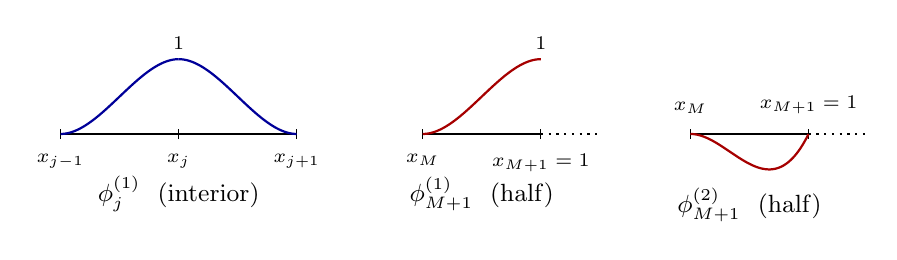
\begin{tikzpicture}[x=1.5cm,y=0.95cm]
  \begin{scope}
  \draw[thick] (0,0) -- (2,0);
  \foreach \i/\lab in {0/{x_{j-1}},1/{x_{j}},2/{x_{j+1}}}{
     \draw (\i,-0.07) -- (\i,0.07);
     \node[below=2pt,font=\scriptsize] at (\i,-0.07) {$\lab$};}
  \draw[thick,blue!60!black,domain=0:1,samples=60,smooth] plot (\x,{3*\x*\x-2*\x*\x*\x});
  \draw[thick,blue!60!black,domain=1:2,samples=60,smooth]
        plot (\x,{3*(2-\x)*(2-\x)-2*(2-\x)*(2-\x)*(2-\x)});
  \node[above,font=\scriptsize] at (1,1) {$1$};
  \node[font=\small] at (1,-0.8) {$\phi^{(1)}_{j}$ \ (interior)};
  \end{scope}
  \begin{scope}[xshift=4.6cm]
  \draw[thick] (0,0) -- (1,0);
  \draw[thick,dotted] (1,0) -- (1.5,0);
  \foreach \i/\lab in {0/{x_{M}},1/{x_{M+1}=1}}{
     \draw (\i,-0.07) -- (\i,0.07);
     \node[below=2pt,font=\scriptsize] at (\i,-0.07) {$\lab$};}
  \draw[thick,red!65!black,domain=0:1,samples=60,smooth] plot (\x,{3*\x*\x-2*\x*\x*\x});
  \node[above,font=\scriptsize] at (1,1) {$1$};
  \node[font=\small] at (0.5,-0.8) {$\phi^{(1)}_{M+1}$ \ (half)};
  \end{scope}
  \begin{scope}[xshift=8.0cm]
  \draw[thick] (0,0) -- (1,0);
  \draw[thick,dotted] (1,0) -- (1.5,0);
  \foreach \i/\lab in {0/{x_{M}},1/{x_{M+1}=1}}{
     \draw (\i,-0.07) -- (\i,0.07);
     \node[above=2pt,font=\scriptsize] at (\i,0.07) {$\lab$};}
  \draw[thick,red!65!black,domain=0:1,samples=60,smooth] plot (\x,{3.2*(\x*\x*(\x-1))});
  \node[font=\small] at (0.5,-0.95) {$\phi^{(2)}_{M+1}$ \ (half)};
  \end{scope}
\end{tikzpicture}
\end{center}

% ------------------------------------------------------------------
\subsection*{Step 3b --- the same thing element by element
  \ \src{Lecture 11 mechanics note: ``$\phi^{(1)}_{j}$ and $\phi^{(2)}_{j}$ are
         the cubic Hermite shape functions $N_{1},N_{2},N_{3},N_{4}$''}}

In a structural code the trial function is written per \emph{element}, not per
node.  It is the same function.  On element $e=[x_{e-1},x_{e}]$, with
$t=x-x_{e-1}$,
\[
  U\big|_{e}=N_{1}w_{e-1}+N_{2}\theta_{e-1}+N_{3}w_{e}+N_{4}\theta_{e},
  \qquad
  \begin{aligned}
    N_{1}&=1-3\tfrac{t^{2}}{h^{2}}+2\tfrac{t^{3}}{h^{3}}, &
    N_{2}&=t-2\tfrac{t^{2}}{h}+\tfrac{t^{3}}{h^{2}},\\
    N_{3}&=3\tfrac{t^{2}}{h^{2}}-2\tfrac{t^{3}}{h^{3}}, &
    N_{4}&=-\tfrac{t^{2}}{h}+\tfrac{t^{3}}{h^{2}} .
  \end{aligned}
\]
Comparing with \eqref{eq:phi1}--\eqref{eq:phi2}: $\phi^{(1)}_{j}$ is $N_{3}$ on
the element to its left and $N_{1}$ on the element to its right;
$\phi^{(2)}_{j}$ is $N_{4}$ then $N_{2}$.  One global basis function $=$ two
element shape functions glued at the node, and the coefficients are the same
numbers, $w_{e}=\xi_{e}$, $\theta_{e}=\eta_{e}$ --- which is why assembling
element matrices into global slots (Step 5) works.
% ------------------------------------------------------------------
\subsection*{Step 4 --- the CG(3) method
  \ \src{Lecture 11 box; Lecture 12, eq.~(1.181): trial $U$, test $=$ each basis
         function}}

\begin{steps}
\item \textbf{Trial function:}
\begin{equation}\label{eq:trial}
  U(x)=\sum_{j=1}^{M+1}\xi_{j}\,\phi^{(1)}_{j}(x)+\sum_{j=1}^{M+1}\eta_{j}\,\phi^{(2)}_{j}(x),
  \qquad \xi_{j}=U(x_{j}),\quad \eta_{j}=U'(x_{j}).
\end{equation}
\item \textbf{Test functions:} $v=\phi^{(1)}_{k},\phi^{(2)}_{k}$, $k=1,\dots,M+1$.
\end{steps}

\medskip
\noindent\fbox{\parbox{0.955\linewidth}{%
\textbf{(CG(3) FEM)}\ \ Find $U\in V_{h}$ such that
$\displaystyle\int_{0}^{1}U''v''\dx=\int_{0}^{1}fv\dx$ for all $v\in V_{h}$.}}

% ------------------------------------------------------------------
\subsection*{Step 5 --- the linear system
  \ \src{Lecture 12, eqs.~(1.189)--(1.194): the $\bm{A},\bm{B},\bm{C}$ blocks}}

\begin{steps}
\item Substituting \eqref{eq:trial} and testing against each basis function
      gives $2(M+1)$ equations in the $2(M+1)$ unknowns $\xi,\eta$.  Sorting them by
      \emph{type} of DOF gives Lecture 12's block form
\begin{equation}\label{eq:system}
  \underbrace{\left[\begin{array}{c|c}\bm{A}&\bm{C}\\\hline \bm{C}^{T}&\bm{B}\end{array}\right]}_{\bm{S}\,\in\,\mathbb{R}^{2(M+1)\times2(M+1)}}
  \left[\begin{array}{c}\bm{\xi}\\\hline\bm{\eta}\end{array}\right]
  =\left[\begin{array}{c}\bm{b}^{(1)}\\\hline\bm{b}^{(2)}\end{array}\right],
\end{equation}
\[
  A_{kj}=\int_{0}^{1}\bigl(\phi^{(1)}_{j}\bigr)''\bigl(\phi^{(1)}_{k}\bigr)''\dx,\quad
  B_{kj}=\int_{0}^{1}\bigl(\phi^{(2)}_{j}\bigr)''\bigl(\phi^{(2)}_{k}\bigr)''\dx,\quad
  C_{kj}=\int_{0}^{1}\bigl(\phi^{(2)}_{j}\bigr)''\bigl(\phi^{(1)}_{k}\bigr)''\dx .
\]
\item On a uniform mesh these are Lecture 12's matrices --- \textbf{except in the
      last row and column}, where node $M+1$ collects only \emph{one} element
      instead of two:
\begin{equation}\label{eq:blocks}
  \bm{A}=\frac{12}{h^{3}}\!\begin{bmatrix}
   2&-1& & \\ -1&2&\ddots& \\ &\ddots&2&-1\\ & &-1&\boxed{1}\end{bmatrix}\!,\quad
  \bm{B}=\frac{2}{h}\!\begin{bmatrix}
   4&1& & \\ 1&4&\ddots& \\ &\ddots&4&1\\ & &1&\boxed{2}\end{bmatrix}\!,\quad
  \bm{C}=\frac{6}{h^{2}}\!\begin{bmatrix}
   0&1& & \\ -1&0&\ddots& \\ &\ddots&0&1\\ & &-1&\boxed{-1}\end{bmatrix}\!.
\end{equation}
\item All three are $(M+1)\times(M+1)$ and tridiagonal; $\bm{A},\bm{B}$ symmetric,
      $\bm{C}^{T}=-\bm{C}$ \emph{except} for its last diagonal entry, so
      $\bm{S}$ is symmetric and --- since $V_{h}\subset V$ has no rigid-body
      mode left after clamping --- positive definite.
\end{steps}

\medskip
{\small\color{black!60}\textbf{Why the boxed entries.}  Exactly Lecture 6's
argument for the Neumann end node (``the last diagonal entry is $1$, not $2$'':
every interior node has two elements attached, the end node only one).  Writing
the Hermite element matrix with $EI=1$,
$\frac{1}{h^{3}}\left[\begin{smallmatrix}12&6h&-12&6h\\6h&4h^{2}&-6h&2h^{2}\\
-12&-6h&12&-6h\\6h&2h^{2}&-6h&4h^{2}\end{smallmatrix}\right]$,
an interior node collects $12+12=24$, $4h^{2}+4h^{2}=8h^{2}$ and
$-6h+6h=0$; the tip collects only the left element's $12$, $4h^{2}$ and $-6h$.
That is $\boxed{1}$, $\boxed{2}$ and $\boxed{-1}$ in the scalings of
\eqref{eq:blocks}.}

% ------------------------------------------------------------------
\subsection*{Step 6 --- the load vector
  \ \src{Lecture 12, eqs.~(1.195)--(1.198)}}

\begin{steps}
\item By definition,
\begin{equation}\label{eq:load}
  b^{(1)}_{k}=\int_{0}^{1}f\,\phi^{(1)}_{k}\dx,
  \qquad
  b^{(2)}_{k}=\int_{0}^{1}f\,\phi^{(2)}_{k}\dx,
  \qquad k=1,\dots,M+1 .
\end{equation}
\item Lecture 12 evaluates these by interpolating the load with the same Hermite
      basis.  For an \emph{interior} node $k\le M$ that gives (1.197)--(1.198),
\begin{align*}
  b^{(1)}_{k}&=\tfrac{h}{70}\bigl[9f_{k-1}+52f_{k}+9f_{k+1}\bigr]
             +\tfrac{13h^{2}}{420}\bigl[f'_{k-1}-f'_{k+1}\bigr],\\
  b^{(2)}_{k}&=\tfrac{13h^{2}}{420}\bigl[f_{k+1}-f_{k-1}\bigr]
             -\tfrac{h^{3}}{420}\bigl[3f'_{k-1}-8f'_{k}+3f'_{k+1}\bigr].
\end{align*}
\item At the \textbf{tip} $k=M+1$ every term carrying $x_{M+2}$ is absent, and
      only the left element contributes:
\begin{align*}
  b^{(1)}_{M+1}&=\tfrac{h}{420}\bigl[54f_{M}+156f_{M+1}\bigr]
             +\tfrac{h^{2}}{420}\bigl[13f'_{M}-22f'_{M+1}\bigr],\\
  b^{(2)}_{M+1}&=-\tfrac{h^{2}}{420}\bigl[13f_{M}+22f_{M+1}\bigr]
             -\tfrac{h^{3}}{420}\bigl[3f'_{M}-4f'_{M+1}\bigr].
\end{align*}
\item (In Problem 6 the integrals \eqref{eq:load} are evaluated by Gauss
      quadrature instead, which avoids interpolating $f$ at all.)
\end{steps}

\medskip
{\small\color{black!60}\textbf{Mechanics reading.}  $\bm{\xi}$ are nodal
deflections, $\bm{\eta}$ nodal rotations, $\bm{b}^{(1)}$ consistent nodal forces
and $\bm{b}^{(2)}$ consistent nodal moments.  \eqref{eq:blocks} is the standard
Euler--Bernoulli beam assembly with $EI=1$, sorted by DOF type rather than by
node.  The free tip keeps both DOFs and gets a half-stiffness row --- which is
just the statement that only one element frames into it.}

% ==================================================================
\newpage
\section*{Problem 4}

\textbf{Problem.} Prove an \emph{a priori} error estimate for this method in the
energy norm
\[
  \norm{e}_{E}=\Bigl\{\int_{0}^{1}(e'')^{2}\dx\Bigr\}^{1/2} .
\]

\medskip
{\small\color{black!60}Throughout, $e:=u-U$ (exact minus FEM).  Two norms, told
apart by the subscript:
$\norm{v}_{E}=\bigl(\int_{0}^{1}(v'')^{2}\dx\bigr)^{1/2}$ (energy, the one asked
for) and $\norm{v}=\bigl(\int_{0}^{1}v^{2}\dx\bigr)^{1/2}$ ($L^{2}$).  Note
$\norm{v}_{E}=\norm{v''}$: the energy norm is just the $L^{2}$ norm of the
curvature.  Lectures 6--7 carry a coefficient $a$ in these; here $a\equiv1$.}

% ------------------------------------------------------------------
\subsection*{Step 1 --- Galerkin orthogonality
  \ \src{Lecture 6, eq.~(1.95): write both problems, subtract}}

\begin{steps}
\item The exact solution satisfies \eqr{eq:weak} against \emph{every} $v\in V$:
\[
  \int_{0}^{1}u''v''\dx=\int_{0}^{1}fv\dx\qquad\forall\,v\in V .
\]
\item The FEM solution satisfies the same identity, but only against
      $v\in V_{h}$:
\[
  \int_{0}^{1}U''v''\dx=\int_{0}^{1}fv\dx\qquad\forall\,v\in V_{h}.
\]
\item $V_{h}\subset V$, so the first line is also true for every $v\in V_{h}$.
      Subtract, for those $v$ --- the right-hand sides are identical and cancel:
\begin{equation}\label{eq:GO}
  \boxed{\;\int_{0}^{1}e''\,v''\dx=0\qquad\text{for all }v\in V_{h},
  \qquad e=u-U\;}
\end{equation}
\end{steps}

\medskip
{\small\color{black!60}Conforming ($V_{h}\subset V$) is what makes the
subtraction legal: without it the exact solution's identity would not be
available for the $v$ we want to use.}

% ------------------------------------------------------------------
\subsection*{Step 2 --- Cauchy's inequality, in the form needed here
  \ \src{Lecture 6, eq.~(1.91)}}

\begin{steps}
\item Lecture 6 states it as
      $\bigl|\int_{0}^{1}a\,v'w'\dx\bigr|\le\norm{v}_{E}\norm{w}_{E}$.
\item For this problem the pairing is of \emph{second} derivatives with
      $a\equiv1$, so the same inequality reads
\begin{equation}\label{eq:cauchy}
  \boxed{\;\Bigl|\int_{0}^{1}v''w''\dx\Bigr|\le\norm{v}_{E}\,\norm{w}_{E}\;}
  \qquad
  \norm{v}_{E}=\Bigl(\int_{0}^{1}(v'')^{2}\dx\Bigr)^{1/2},\ \
  \norm{w}_{E}=\Bigl(\int_{0}^{1}(w'')^{2}\dx\Bigr)^{1/2}.
\end{equation}
\end{steps}

% ------------------------------------------------------------------
\subsection*{Step 3 --- $U$ is the best approximation in the energy norm
  \ \src{Lecture 6, eqs.~(1.96)--(1.100): insert $-v+v$, kill one term by
         \eqref{eq:GO}, apply Cauchy, cancel one factor}}

\begin{steps}
\item Start from the definition, both factors $e$:
\[
  \norm{e}_{E}^{2}=\int_{0}^{1}e''\,e''\dx .
\]
\item Pick \emph{any} $v\in V_{h}$ and insert $-v+v$ in the second factor,
      $e=u-U=(u-v)+(v-U)$:
\begin{equation}\label{eq:split}
  \norm{e}_{E}^{2}
  =\int_{0}^{1}e''(u-v)''\dx
  +\underbrace{\int_{0}^{1}e''(v-U)''\dx}_{=\;0\ \text{by \eqref{eq:GO}}} .
\end{equation}
\item \textbf{Why the second integral vanishes.}  \eqref{eq:GO} kills
      $\int e''\,(\,\cdot\,)''$ against anything \emph{in $V_{h}$}.  Here
      $v\in V_{h}$ and $U\in V_{h}$, so $v-U\in V_{h}$ and the integral is zero.
      Note $u-v$ is \emph{not} in $V_{h}$ ($u$ is not a piecewise cubic) ---
      that is exactly why the split puts $v-U$ in the slot being annihilated.
\item So for any $v\in V_{h}$, $\ \norm{e}_{E}^{2}=\int_{0}^{1}e''(u-v)''\dx$.
      Apply \eqref{eq:cauchy}:
\[
  \norm{e}_{E}^{2}\;\le\;\norm{e}_{E}\,\norm{u-v}_{E}.
\]
\item Cancel one factor $\norm{e}_{E}$ (if it is zero, $U=u$ in the energy norm
      and there is nothing to prove):
\begin{equation}\label{eq:best}
  \boxed{\;\norm{u-U}_{E}\;\le\;\norm{u-v}_{E}\qquad\text{for every }v\in V_{h}\;}
\end{equation}
\end{steps}

\medskip
{\small\color{black!60}\eqref{eq:best} says the FEM solution is the
\textbf{closest} member of $V_{h}$ to $u$ in the energy norm --- no other
piecewise cubic on this mesh stores its bending energy more accurately.  The
constant is exactly $1$.  The error of the \emph{method} is now bounded by the
error of \emph{interpolation}, which has nothing to do with the method and
everything to do with the mesh.}

% ------------------------------------------------------------------
\subsection*{Step 4 --- choose $v$ to be the interpolant
  \ \src{Lecture 12, eq.~(1.182): $\Pi_h u$ matches $u$ \emph{and} $u'$ at every
         node}}

\begin{steps}
\item \eqref{eq:best} holds for \emph{every} $v\in V_{h}$, so we are free to
      pick the most convenient one.  Take the Hermite interpolant
\begin{equation}\label{eq:interp}
  \Pi_{h}u=\sum_{j=1}^{M+1}u(x_{j})\,\phi^{(1)}_{j}
          +\sum_{j=1}^{M+1}u'(x_{j})\,\phi^{(2)}_{j},
\end{equation}
      the piecewise cubic that agrees with $u$ in \emph{value and slope} at
      every node.
\item \textbf{Check $\Pi_{h}u\in V_{h}$.}  Every $\phi$ in \eqref{eq:interp}
      vanishes together with its slope at $x_{0}=0$, so
      $\Pi_{h}u(0)=(\Pi_{h}u)'(0)=0$: the essential BCs hold, and $\Pi_{h}u$ is
      a legal choice.  (Node $0$ is absent from the sums, but $u(0)=u'(0)=0$
      anyway, so $\Pi_{h}u$ still interpolates $u$ at \emph{all} $M+2$ nodes.)
\item Put $v=\Pi_{h}u$ into \eqref{eq:best}:
\begin{equation}\label{eq:toint}
  \norm{u-U}_{E}\;\le\;\norm{u-\Pi_{h}u}_{E}
  \;=\;\norm{\bigl(u-\Pi_{h}u\bigr)''} .
\end{equation}
\end{steps}

% ------------------------------------------------------------------
\subsection*{Step 5 --- insert the interpolation estimate
  \ \src{Lecture 12, eq.~(1.185):
         $\norm{(u-\Pi_h u)''}\le c_{3}\norm{h^{2}u^{(4)}}$}}

\begin{steps}
\item Lecture 12 states the three Hermite interpolation errors; the one that
      matches \eqref{eq:toint} is the second-derivative line,
\begin{equation}\label{eq:int2}
  \norm{\bigl(u-\Pi_{h}u\bigr)''}_{L^{2}(0,1)}
  \;\le\;c_{3}\,\norm{h^{2}u^{(4)}}_{L^{2}(0,1)} .
\end{equation}
\item Combining \eqref{eq:toint} and \eqref{eq:int2}:
\begin{equation}\label{eq:result}
  \boxed{\;\norm{u-U}_{E}\;\le\;c_{3}\,\norm{h^{2}u^{(4)}}\;}
\end{equation}
\item On a uniform mesh $h$ is a constant and comes out of the norm:
\begin{equation}\label{eq:resultuni}
  \boxed{\;\norm{u-U}_{E}\;\le\;c_{3}\,h^{2}\,\norm{u^{(4)}}
  \;=\;\mathcal{O}(h^{2})\;}
\end{equation}
\end{steps}

\medskip
\noindent\fbox{\parbox{0.955\linewidth}{%
\textbf{Result.}  For CG(3) on the cantilever, with $u^{(4)}=f$ square
integrable,
\[
  \norm{u-U}_{E}=\Bigl\{\int_{0}^{1}\bigl((u-U)''\bigr)^{2}\dx\Bigr\}^{1/2}
  \;\le\;c_{3}\,h^{2}\,\norm{u^{(4)}} ,
\]
\ie\ the energy-norm error converges at \textbf{second order} in $h$.  Halving
the mesh divides the error by $4$.}}

\medskip
{\small\color{black!60}\textbf{Reading the result.}  The energy norm measures
the error in $u''$, the \emph{curvature} --- and curvature is bending moment
($M=EI\,u''$).  So this is the convergence rate of the \emph{moment/stress}
field, $O(h^{2})$.  Problem 5 does the displacement, which will turn out two
orders better.  Note also $u^{(4)}=f$ by the PDE, so the bound can be written
$c_{3}h^{2}\norm{f}$: the rougher the load, the worse the constant, and if $f$
is not square integrable the estimate says nothing.}

% ==================================================================
\newpage
\section*{Problem 5}

\textbf{Problem.} Prove an \emph{a priori} error estimate for this method in the
$L^{2}$ norm
\[
  \norm{e}_{L^{2}}=\Bigl\{\int_{0}^{1}(e)^{2}\dx\Bigr\}^{1/2} .
\]

\medskip
{\small\color{black!60}Written $\norm{e}$ below.  The energy norm measured
$e''$; this one measures $e$ itself.  The whole point is that it converges
\emph{faster}, and the device that proves it is the duality argument of
Lectures 7--8.}

% ------------------------------------------------------------------
\subsection*{Step 1 --- the dual problem
  \ \src{Lecture 7, eq.~(1.108): an auxiliary BVP whose \emph{load is the error
         itself}}}

\begin{steps}
\item Lecture 7 solves $-(a\phi')'=e$ for the second-order problem.  The beam
      operator is $\mathrm{d}^{4}/\mathrm{d}x^{4}$, so the same device reads
\begin{equation}\label{eq:dual}
  \boxed{\;\phi^{(iv)}=e\ \text{ on }(0,1),
  \qquad \phi(0)=\phi'(0)=0,\qquad \phi''(1)=\phi'''(1)=0\;}
\end{equation}
      --- the \emph{same} cantilever BCs as the original problem.
\item As in Lecture 7, this is legitimate because the problem is
      \textbf{self-adjoint}: the dual operator is the same $(\cdot)^{(iv)}$, so
      we are not obliged to solve a different equation.
\item $\phi$ is never computed.  It exists only to be paired against $e$, which
      is the next step.
\end{steps}

% ------------------------------------------------------------------
\subsection*{Step 2 --- turn $\norm{e}^{2}$ into an integral of $e''\phi''$
  \ \src{Lecture 7, eq.~(1.109): multiply the dual equation by $e$, integrate by
         parts, boundary terms vanish}}

\begin{steps}
\item Multiply \eqref{eq:dual} by $e$ and integrate --- the load of the dual
      problem is $e$, so this manufactures $\norm{e}^{2}$ on the left:
\[
  \norm{e}^{2}=\int_{0}^{1}e\,e\dx=\int_{0}^{1}e\,\phi^{(iv)}\dx .
\]
\item Integrate by parts twice, exactly as in Problem 1:
\begin{equation}\label{eq:dualibp}
  \int_{0}^{1}e\,\phi^{(iv)}\dx
   =\underbrace{\Bigl[e\,\phi'''\Bigr]_{0}^{1}}_{\text{A}}
   -\underbrace{\Bigl[e'\,\phi''\Bigr]_{0}^{1}}_{\text{B}}
   +\int_{0}^{1}e''\,\phi''\dx .
\end{equation}
\item All four boundary halves vanish --- but for two \emph{different} reasons:
\end{steps}

\begin{center}\small
\renewcommand{\arraystretch}{1.3}
\begin{tabular}{@{}lll@{}}
\toprule
term & dies because & which function supplies it\\
\midrule
$e(1)\,\phi'''(1)$ & $\phi'''(1)=0$, a \emph{natural} BC of \eqref{eq:dual} & the dual $\phi$\\
$e'(1)\,\phi''(1)$ & $\phi''(1)=0$, a \emph{natural} BC of \eqref{eq:dual} & the dual $\phi$\\
$e(0)\,\phi'''(0)$ & $e(0)=u(0)-U(0)=0-0=0$ & the error $e$\\
$e'(0)\,\phi''(0)$ & $e'(0)=u'(0)-U'(0)=0-0=0$ & the error $e$\\
\bottomrule
\end{tabular}
\end{center}

\begin{steps}
\item (The $x=0$ rows hold because \emph{both} $u$ and $U$ lie in $V$, so each
      has zero value and zero slope at the clamped end; their difference does
      too.)  Hence
\begin{equation}\label{eq:esq}
  \norm{e}^{2}=\int_{0}^{1}e''\,\phi''\dx .
\end{equation}
\end{steps}

% ------------------------------------------------------------------
\subsection*{Step 3 --- subtract zero, using Galerkin orthogonality
  \ \src{Lecture 7, eq.~(1.111): replace $\phi$ by the interpolation error
         $\phi-\Pi_h\phi$}}

\begin{steps}
\item $\Pi_{h}\phi\in V_{h}$ (same check as Problem 4: $\phi(0)=\phi'(0)=0$), so
      \eqref{eq:GO} gives $\int_{0}^{1}e''(\Pi_{h}\phi)''\dx=0$.
\item Subtract that zero from \eqref{eq:esq}:
\begin{equation}\label{eq:dualGO}
  \norm{e}^{2}
   =\int_{0}^{1}e''\phi''\dx-\underbrace{\int_{0}^{1}e''(\Pi_{h}\phi)''\dx}_{=\,0}
   =\int_{0}^{1}e''\bigl(\phi-\Pi_{h}\phi\bigr)''\dx .
\end{equation}
\end{steps}

\medskip
{\small\color{black!60}\textbf{This single move is the whole trick.}  Nothing
was added or removed --- the subtracted term is zero.  But $\phi''$ is not
small, whereas the \emph{interpolation error} $(\phi-\Pi_{h}\phi)''$ is: it is
$O(h^{2})$.  That substitution is what buys the extra powers of $h$.}

% ------------------------------------------------------------------
\subsection*{Step 4 --- Cauchy, then interpolation, then the dual equation
  \ \src{Lecture 6 eq.~(1.91) and Lecture 12 eq.~(1.185), as in Problem 4}}

\begin{steps}
\item Cauchy \eqref{eq:cauchy} on \eqref{eq:dualGO}:
\[
  \norm{e}^{2}\;\le\;\norm{e''}\,\bigl\|\bigl(\phi-\Pi_{h}\phi\bigr)''\bigr\|
  \;=\;\norm{e}_{E}\,\bigl\|\bigl(\phi-\Pi_{h}\phi\bigr)''\bigr\| .
\]
\item Lecture 12's interpolation estimate \eqref{eq:int2}, now applied to $\phi$
      instead of $u$:
\[
  \bigl\|\bigl(\phi-\Pi_{h}\phi\bigr)''\bigr\|\;\le\;c_{3}\,h^{2}\,\norm{\phi^{(4)}} .
\]
\item \textbf{Here the dual problem pays off.}  $\phi^{(iv)}=e$ by
      \eqref{eq:dual}, so $\norm{\phi^{(4)}}=\norm{e}$ \emph{exactly} --- no
      stability constant is needed.  (Lecture 7 needs $S_{a}$ because of the
      coefficient $a$; its own note records that for $a\equiv$ const the ratio
      is explicit.  Here the coefficient is $1$ and the dual load \emph{is} the
      error, so the constant is $1$.)
\item Therefore
\[
  \norm{e}^{2}\;\le\;c_{3}\,h^{2}\,\norm{e}_{E}\,\norm{e},
\]
      and cancelling one factor $\norm{e}$ (if it is zero there is nothing to
      prove):
\begin{equation}\label{eq:L2toE}
  \boxed{\;\norm{e}\;\le\;c_{3}\,h^{2}\,\norm{e}_{E}\;}
\end{equation}
\end{steps}

% ------------------------------------------------------------------
\subsection*{Step 5 --- insert Problem 4}

\begin{steps}
\item Problem 4 gave $\norm{e}_{E}\le c_{3}h^{2}\norm{u^{(4)}}$,
      \eqref{eq:resultuni}.  Substituting into \eqref{eq:L2toE}:
\begin{equation}\label{eq:L2result}
  \boxed{\;\norm{e}_{L^{2}}\;\le\;c_{3}^{2}\,h^{4}\,\norm{u^{(4)}}
  \;=\;\mathcal{O}(h^{4})\;}
\end{equation}
\end{steps}

\medskip
\noindent\fbox{\parbox{0.955\linewidth}{%
\textbf{Result.}  For CG(3) on the cantilever,
\[
  \norm{u-U}_{E}\le c_{3}h^{2}\norm{u^{(4)}}=\mathcal{O}(h^{2}),
  \qquad
  \norm{u-U}_{L^{2}}\le c_{3}^{2}h^{4}\norm{u^{(4)}}=\mathcal{O}(h^{4}).
\]
The $L^{2}$ error converges \textbf{two orders faster} than the energy-norm
error.}}

\medskip
{\small\color{black!60}\textbf{Where the two extra powers came from.}  The
interpolation estimate was used \emph{twice}: once on $e$ through Problem 4, and
once on $\phi$ through \eqref{eq:dualGO}.  Each contributes $h^{2}$.  This is the
duality (Aubin--Nitsche) argument of Lecture 7, one order higher because the
beam's interpolation estimate carries $h^{2}$ where the bar's carried $h$.

\textbf{Engineering reading.}  Displacements converge far faster than moments.
$\norm{e}_{E}$ measures curvature, \ie\ bending moment: $O(h^{2})$.
$\norm{e}_{L^{2}}$ measures deflection: $O(h^{4})$.  On a mesh where the
deflection plot looks perfectly converged, the moment plot can still be visibly
wrong --- which is why stress, not displacement, drives mesh refinement.  These
are the two rates Problem 6 measures numerically.}

\end{document}
